% Options for packages loaded elsewhere
\PassOptionsToPackage{unicode}{hyperref}
\PassOptionsToPackage{hyphens}{url}
\documentclass[
  11pt,
]{ctexart}
\usepackage{xcolor}
\usepackage[margin=2.3cm]{geometry}
\usepackage{amsmath,amssymb}
\setcounter{secnumdepth}{-\maxdimen} % remove section numbering
\usepackage{iftex}
\ifPDFTeX
  \usepackage[T1]{fontenc}
  \usepackage[utf8]{inputenc}
  \usepackage{textcomp} % provide euro and other symbols
\else % if luatex or xetex
  \usepackage{unicode-math} % this also loads fontspec
  \defaultfontfeatures{Scale=MatchLowercase}
  \defaultfontfeatures[\rmfamily]{Ligatures=TeX,Scale=1}
\fi
\usepackage{lmodern}
\ifPDFTeX\else
  % xetex/luatex font selection
\fi
% Use upquote if available, for straight quotes in verbatim environments
\IfFileExists{upquote.sty}{\usepackage{upquote}}{}
\IfFileExists{microtype.sty}{% use microtype if available
  \usepackage[]{microtype}
  \UseMicrotypeSet[protrusion]{basicmath} % disable protrusion for tt fonts
}{}
\makeatletter
\@ifundefined{KOMAClassName}{% if non-KOMA class
  \IfFileExists{parskip.sty}{%
    \usepackage{parskip}
  }{% else
    \setlength{\parindent}{0pt}
    \setlength{\parskip}{6pt plus 2pt minus 1pt}}
}{% if KOMA class
  \KOMAoptions{parskip=half}}
\makeatother
\usepackage{color}
\usepackage{fancyvrb}
\newcommand{\VerbBar}{|}
\newcommand{\VERB}{\Verb[commandchars=\\\{\}]}
\DefineVerbatimEnvironment{Highlighting}{Verbatim}{commandchars=\\\{\}}
% Add ',fontsize=\small' for more characters per line
\newenvironment{Shaded}{}{}
\newcommand{\AlertTok}[1]{\textcolor[rgb]{1.00,0.00,0.00}{\textbf{#1}}}
\newcommand{\AnnotationTok}[1]{\textcolor[rgb]{0.38,0.63,0.69}{\textbf{\textit{#1}}}}
\newcommand{\AttributeTok}[1]{\textcolor[rgb]{0.49,0.56,0.16}{#1}}
\newcommand{\BaseNTok}[1]{\textcolor[rgb]{0.25,0.63,0.44}{#1}}
\newcommand{\BuiltInTok}[1]{\textcolor[rgb]{0.00,0.50,0.00}{#1}}
\newcommand{\CharTok}[1]{\textcolor[rgb]{0.25,0.44,0.63}{#1}}
\newcommand{\CommentTok}[1]{\textcolor[rgb]{0.38,0.63,0.69}{\textit{#1}}}
\newcommand{\CommentVarTok}[1]{\textcolor[rgb]{0.38,0.63,0.69}{\textbf{\textit{#1}}}}
\newcommand{\ConstantTok}[1]{\textcolor[rgb]{0.53,0.00,0.00}{#1}}
\newcommand{\ControlFlowTok}[1]{\textcolor[rgb]{0.00,0.44,0.13}{\textbf{#1}}}
\newcommand{\DataTypeTok}[1]{\textcolor[rgb]{0.56,0.13,0.00}{#1}}
\newcommand{\DecValTok}[1]{\textcolor[rgb]{0.25,0.63,0.44}{#1}}
\newcommand{\DocumentationTok}[1]{\textcolor[rgb]{0.73,0.13,0.13}{\textit{#1}}}
\newcommand{\ErrorTok}[1]{\textcolor[rgb]{1.00,0.00,0.00}{\textbf{#1}}}
\newcommand{\ExtensionTok}[1]{#1}
\newcommand{\FloatTok}[1]{\textcolor[rgb]{0.25,0.63,0.44}{#1}}
\newcommand{\FunctionTok}[1]{\textcolor[rgb]{0.02,0.16,0.49}{#1}}
\newcommand{\ImportTok}[1]{\textcolor[rgb]{0.00,0.50,0.00}{\textbf{#1}}}
\newcommand{\InformationTok}[1]{\textcolor[rgb]{0.38,0.63,0.69}{\textbf{\textit{#1}}}}
\newcommand{\KeywordTok}[1]{\textcolor[rgb]{0.00,0.44,0.13}{\textbf{#1}}}
\newcommand{\NormalTok}[1]{#1}
\newcommand{\OperatorTok}[1]{\textcolor[rgb]{0.40,0.40,0.40}{#1}}
\newcommand{\OtherTok}[1]{\textcolor[rgb]{0.00,0.44,0.13}{#1}}
\newcommand{\PreprocessorTok}[1]{\textcolor[rgb]{0.74,0.48,0.00}{#1}}
\newcommand{\RegionMarkerTok}[1]{#1}
\newcommand{\SpecialCharTok}[1]{\textcolor[rgb]{0.25,0.44,0.63}{#1}}
\newcommand{\SpecialStringTok}[1]{\textcolor[rgb]{0.73,0.40,0.53}{#1}}
\newcommand{\StringTok}[1]{\textcolor[rgb]{0.25,0.44,0.63}{#1}}
\newcommand{\VariableTok}[1]{\textcolor[rgb]{0.10,0.09,0.49}{#1}}
\newcommand{\VerbatimStringTok}[1]{\textcolor[rgb]{0.25,0.44,0.63}{#1}}
\newcommand{\WarningTok}[1]{\textcolor[rgb]{0.38,0.63,0.69}{\textbf{\textit{#1}}}}
\usepackage{longtable,booktabs,array}
\newcounter{none} % for unnumbered tables
\usepackage{calc} % for calculating minipage widths
% Correct order of tables after \paragraph or \subparagraph
\usepackage{etoolbox}
\makeatletter
\patchcmd\longtable{\par}{\if@noskipsec\mbox{}\fi\par}{}{}
\makeatother
% Allow footnotes in longtable head/foot
\IfFileExists{footnotehyper.sty}{\usepackage{footnotehyper}}{\usepackage{footnote}}
\makesavenoteenv{longtable}
\usepackage{graphicx}
\makeatletter
\newsavebox\pandoc@box
\newcommand*\pandocbounded[1]{% scales image to fit in text height/width
  \sbox\pandoc@box{#1}%
  \Gscale@div\@tempa{\textheight}{\dimexpr\ht\pandoc@box+\dp\pandoc@box\relax}%
  \Gscale@div\@tempb{\linewidth}{\wd\pandoc@box}%
  \ifdim\@tempb\p@<\@tempa\p@\let\@tempa\@tempb\fi% select the smaller of both
  \ifdim\@tempa\p@<\p@\scalebox{\@tempa}{\usebox\pandoc@box}%
  \else\usebox{\pandoc@box}%
  \fi%
}
% Set default figure placement to htbp
\def\fps@figure{htbp}
\makeatother
\setlength{\emergencystretch}{3em} % prevent overfull lines
\providecommand{\tightlist}{%
  \setlength{\itemsep}{0pt}\setlength{\parskip}{0pt}}
\usepackage{amsmath,amssymb}
\usepackage{pifont}
\usepackage{newunicodechar}
\setCJKmonofont{SimHei}
\newunicodechar{—}{\textemdash{}}
\newunicodechar{α}{\ensuremath{\alpha}}
\newunicodechar{β}{\ensuremath{\beta}}
\newunicodechar{λ}{\ensuremath{\lambda}}
\newunicodechar{μ}{\ensuremath{\mu}}
\newunicodechar{σ}{\ensuremath{\sigma}}
\newunicodechar{ψ}{\ensuremath{\psi}}
\newunicodechar{Δ}{\ensuremath{\Delta}}
\newunicodechar{Σ}{\ensuremath{\Sigma}}
\newunicodechar{±}{\ensuremath{\pm}}
\newunicodechar{−}{\ensuremath{-}}
\newunicodechar{×}{\ensuremath{\times}}
\newunicodechar{·}{\ensuremath{\cdot}}
\newunicodechar{∈}{\ensuremath{\in}}
\newunicodechar{⊆}{\ensuremath{\subseteq}}
\newunicodechar{≤}{\ensuremath{\leq}}
\newunicodechar{≥}{\ensuremath{\geq}}
\newunicodechar{≈}{\ensuremath{\approx}}
\newunicodechar{≡}{\ensuremath{\equiv}}
\newunicodechar{←}{\ensuremath{\leftarrow}}
\newunicodechar{√}{\ensuremath{\surd}}
\newunicodechar{∅}{\ensuremath{\emptyset}}
\newunicodechar{⟨}{\ensuremath{\langle}}
\newunicodechar{⟩}{\ensuremath{\rangle}}
\newunicodechar{²}{\ensuremath{^{2}}}
\newunicodechar{₀}{\ensuremath{_{0}}}
\newunicodechar{§}{\S{}}
\newunicodechar{†}{\ensuremath{\dagger}}
\newunicodechar{✓}{\ding{51}}
\newunicodechar{✗}{\ding{55}}
\newunicodechar{⚠}{\textbf{!}}
\usepackage{bookmark}
\IfFileExists{xurl.sty}{\usepackage{xurl}}{} % add URL line breaks if available
\urlstyle{same}
\hypersetup{
  pdftitle={量子引导贪心算法实验报告},
  hidelinks,
  pdfcreator={LaTeX via pandoc}}

\title{量子引导贪心算法实验报告}
\author{}
\date{}

\begin{document}
\maketitle

\begin{quote}
本报告记录浙江大学量子信息课程项目''量子引导贪心算法''的实验过程与结果。
围绕''CTQW 概率分布能否辅助贪心算法求解最大团问题''这一核心研究问题，
我们设计了四组实验依次验证：前三组在中小规模上确立''CTQW 全局识别有效、
嵌入贪心会被度数覆盖、外置作起点选择器可超越强经典基线''的结论；
第四组借助 Krylov / Chebyshev 近似把 CTQW 起点选择推广到 n=1000+ 的
DIMACS
真实图，验证了方法的\textbf{大规模可行性}，并在专门设计的''度数误导''
图族上展示了 CTQW 相对纯度数信号的\textbf{独有价值}。
\end{quote}

\subsection{1. 工作概述}\label{ux5de5ux4f5cux6982ux8ff0}

\subsubsection{1.1
研究背景与问题陈述}\label{ux7814ux7a76ux80ccux666fux4e0eux95eeux9898ux9648ux8ff0}

\textbf{最大团问题}（Maximum Clique Problem, MCP）是图论中的经典 NP-hard
问题： 给定一张无向图 G=(V, E)，目标是找出最大的节点子集 S⊆V， 使得 S
中任意两个节点之间均存在边相连。该问题在社交网络紧密社群识别、
蛋白质相互作用分析、聚类等场景中均有直接的应用价值；
但由于其计算复杂度，当节点规模稍大时便难以求得精确解。

实际应用中常采用\textbf{贪心算法}进行近似求解：
从某个起始节点出发，每一轮选取一个与当前团内所有节点均相邻的候选节点加入，
直至无法继续扩展为止。算法的核心在于\textbf{每一轮如何挑选下一个节点}------
传统做法依据节点的\textbf{度数}（即邻居数量）进行选择，
但度数本质上是一个局部指标，无法反映图的整体拓扑结构。

由此，本项目的研究问题是：

\begin{quote}
\textbf{能否引入一种感知图全局结构的信号，来辅助贪心算法的判断？
具体而言，连续时间量子游走（CTQW）产生的节点概率分布，
是否可以作为贪心评分函数，提升求解质量？}
\end{quote}

\subsubsection{1.2
算法核心框架}\label{ux7b97ux6cd5ux6838ux5fc3ux6846ux67b6}

\textbf{连续时间量子游走（CTQW）} 可以理解为：
一个量子粒子同时从图上多个节点出发，按照图的连接关系进行幺正演化
\(|\psi(t)\rangle = e^{-iHt}|\psi_0\rangle\)； 最终各节点的概率
\(P_v(t) = |\langle v|\psi(t)\rangle|^2\)
便承载着图的全局结构信号------\textbf{结构越紧密、连接越稠密的区域，
概率集中的程度也越显著}。

基于这一直觉，我们设计\textbf{混合评分函数}：

\[\text{Score}(v, S) = \alpha \cdot Q_{\text{norm}}(v) + (1-\alpha) \cdot R_{\text{norm}}(v)\]

其中 Q 是 CTQW 概率，R 是候选诱导子图度数，α∈{[}0,1{]}
控制量子与经典权重。 α=0 时退化为纯经典贪心，α=1 时为纯量子方案。

\subsubsection{1.3
实验设计与本次工作}\label{ux5b9eux9a8cux8bbeux8ba1ux4e0eux672cux6b21ux5de5ux4f5c}

围绕该框架，我们设计了\textbf{四组实验}依次进行验证：

{\def\LTcaptype{none} % do not increment counter
\begin{longtable}[]{@{}
  >{\raggedright\arraybackslash}p{(\linewidth - 4\tabcolsep) * \real{0.3333}}
  >{\raggedright\arraybackslash}p{(\linewidth - 4\tabcolsep) * \real{0.3333}}
  >{\raggedright\arraybackslash}p{(\linewidth - 4\tabcolsep) * \real{0.3333}}@{}}
\toprule\noalign{}
\begin{minipage}[b]{\linewidth}\raggedright
实验
\end{minipage} & \begin{minipage}[b]{\linewidth}\raggedright
验证问题
\end{minipage} & \begin{minipage}[b]{\linewidth}\raggedright
结论
\end{minipage} \\
\midrule\noalign{}
\endhead
\bottomrule\noalign{}
\endlastfoot
\textbf{实验一} & CTQW 能否识别图的全局团结构？ & \textbf{✓ 成立} \\
\textbf{实验二} & 把 CTQW 嵌入贪心，混合评分是否更稳健？ & \textbf{⚠
部分成立} \\
\textbf{实验三} & 把 CTQW 改作外部起点选择器，能否超越强经典基线？ &
\textbf{✓ 成立} \\
\textbf{实验四} & 借助近似把 CTQW
推广到大规模真实图，量子信号是否仍有价值？ & \textbf{✓
大规模可行；度数误导场景下成立} \\
\end{longtable}
}

主要工程贡献：

\begin{enumerate}
\def\labelenumi{\arabic{enumi}.}
\tightlist
\item
  完成 CTQW 矩阵指数计算 \(|\psi(t)\rangle = e^{-iHt}|\psi_0\rangle\)
  的真实实现（基于 \texttt{scipy.linalg.expm}），替换原有占位代码；
\item
  编写冒烟测试脚本，确认 Hermitian、幺正性、概率守恒等 6 项数值正确性；
\item
  修复 \texttt{DenseCandidateSet} 缺少停止条件的 bug，补全 DS
  任务的停止逻辑；
\item
  累计运行约 \textbf{23,000 次} 算法对比实验，覆盖人工 planted 数据集
  n∈\{30, 50, 100, 150, 200, 300, 500\} 及 DIMACS 真实图（n 至 2000）、
  5 个 α 取值、6 个 λ 取值、5 个 t 取值；
\item
  显著性检验统一采用 Wilcoxon signed-rank paired test， 按 (sample\_id,
  run\_id) 严格配对；
\item
  实现 CTQW 演化的 \textbf{Krylov 子空间}与 \textbf{Chebyshev
  多项式}两种近似
  （\texttt{src/ctqw\_evolution.py}），配合稀疏矩阵-向量乘法与超时隔离
  （\texttt{src/timeout.py}），将 CTQW 起点选择推广到 n=1000+
  的大规模真实图；
\item
  新增 \textbf{度数误导（degree-misleading）数据生成器}
  （\texttt{datasets/generate\_misleading.py}）：诱饵节点度数虚高却进不了团，
  用于在''度数信号失效''的图族上检验 CTQW 的独立价值。
\end{enumerate}

\subsection{2.
实验环境与实现说明}\label{ux5b9eux9a8cux73afux5883ux4e0eux5b9eux73b0ux8bf4ux660e}

\subsubsection{2.1 软件环境}\label{ux8f6fux4ef6ux73afux5883}

\begin{itemize}
\tightlist
\item
  Python 3.13
\item
  NumPy 2.4 / SciPy 1.17 / NetworkX 3.6 / Matplotlib 3.11 / Pandas 3.0
\end{itemize}

\subsubsection{2.2 CTQW
演化的实现}\label{ctqw-ux6f14ux5316ux7684ux5b9eux73b0}

按理论文档 §5 §6 定义，单轮 CTQW 概率计算流程：

\begin{Shaded}
\begin{Highlighting}[]
\NormalTok{H }\OperatorTok{=}\NormalTok{ construct\_hamiltonian(adjacency, S, lam)   }\CommentTok{\# H = A + λ·Σ|u⟩⟨u|}
\NormalTok{psi0 }\OperatorTok{=}\NormalTok{ build\_initial\_state(n, S, adjacency, init\_method)}
\NormalTok{U }\OperatorTok{=}\NormalTok{ scipy.linalg.expm(}\OperatorTok{{-}}\OtherTok{1j} \OperatorTok{*}\NormalTok{ H }\OperatorTok{*}\NormalTok{ t)             }\CommentTok{\# 演化算子}
\NormalTok{psi\_t }\OperatorTok{=}\NormalTok{ U }\OperatorTok{@}\NormalTok{ psi0                               }\CommentTok{\# 状态演化}
\NormalTok{probs }\OperatorTok{=}\NormalTok{ np.}\BuiltInTok{abs}\NormalTok{(psi\_t) }\OperatorTok{**} \DecValTok{2}                     \CommentTok{\# 概率 P\_v = |ψ\_v|²}
\end{Highlighting}
\end{Shaded}

\subsubsection{2.3
数值正确性验证}\label{ux6570ux503cux6b63ux786eux6027ux9a8cux8bc1}

冒烟测试在 \texttt{mc\_n30\_p01\_k5\_000} 实例上检查 6 项：

{\def\LTcaptype{none} % do not increment counter
\begin{longtable}[]{@{}ll@{}}
\toprule\noalign{}
检查项 & 结果 \\
\midrule\noalign{}
\endhead
\bottomrule\noalign{}
\endlastfoot
H = H† （Hermitian） & max\textbar H − H†\textbar{} = 0.00 \\
U†U = I （幺正性） & max\textbar U†U − I\textbar{} ≈
1e-15（机器精度） \\
Σ P\_v = 1 （概率守恒） & 误差 \textless{} 1e-15 \\
P\_v ≥ 0 （概率非负） & min P\_v = 7.22e-4 \\
Ratio \textgreater{} 1 （团节点概率高于背景） & 最高 Ratio = 9.43 \\
QuantumGuidedGreedy 端到端 & 精确找到植入团 \{12,13,24,27,28\} \\
\end{longtable}
}

\textbf{6 项全部通过，CTQW 实现数值上正确}。

\subsection{3. 实验一：CTQW
概率分布可视化}\label{ux5b9eux9a8cux4e00ctqw-ux6982ux7387ux5206ux5e03ux53efux89c6ux5316}

\subsubsection{3.1 实验目的}\label{ux5b9eux9a8cux76eeux7684}

在将 CTQW 引入贪心算法之前，首先需要验证最基础的前提： \textbf{CTQW
演化之后，植入团节点的概率是否显著高于背景节点？} 即 CTQW
是否真的具备识别图的全局团结构的能力？

\subsubsection{3.2 实验设置}\label{ux5b9eux9a8cux8bbeux7f6e}

\begin{itemize}
\tightlist
\item
  数据：\texttt{mc\_n30\_p01\_k5\_000.json}（30 节点、边密度 p=0.1、植入
  5-团）
\item
  参数：t=1.0, λ=0.5, init=uniform
\item
  评价指标：\(\text{Ratio} = \dfrac{\text{Mean}(P_v, v \in S_{\text{target}})}{\text{Mean}(P_v, v \notin S_{\text{target}})}\)
\end{itemize}

\subsubsection{3.3 实验结果}\label{ux5b9eux9a8cux7ed3ux679c}

{\def\LTcaptype{none} % do not increment counter
\begin{longtable}[]{@{}ll@{}}
\toprule\noalign{}
指标 & 数值 \\
\midrule\noalign{}
\endhead
\bottomrule\noalign{}
\endlastfoot
目标节点（5 个团节点）平均概率 & \textbf{0.1172} \\
背景节点（25 个）平均概率 & \textbf{0.0166} \\
\textbf{Ratio} & \textbf{7.08} \\
\end{longtable}
}

可视化图（保存于 \texttt{results/exp1\_ctqw\_visualization/}）：

\begin{itemize}
\tightlist
\item
  \texttt{mc\_n30\_p01\_k5\_000\_t1.0\_lam0.5\_prob.png}：
  左图为节点图（红色团节点显著更大），右图为概率直方图；
\item
  \texttt{mc\_n30\_p01\_k5\_000\_t1.0\_lam0.5\_compare.png}： 度数 vs
  CTQW 概率散点图，\textbf{5 个团节点全部位于 y=x 对角线上方}。
\end{itemize}

\subsubsection{3.4 结论}\label{ux7ed3ux8bba}

CTQW 在植入团区域形成了明显的概率集中（团节点平均概率约为背景节点的 7
倍）， 且团节点的 CTQW 概率''超出''其度数信号------ 证明 CTQW
\textbf{提供了独立于度数之外的全局结构信息}。

\begin{quote}
\textbf{实验一结论：CTQW 具备识别图全局团结构的能力，假设成立。}
\end{quote}

\subsection{4. 实验二：CTQW
嵌入贪心算法的稳健性验证}\label{ux5b9eux9a8cux4e8cctqw-ux5d4cux5165ux8d2aux5fc3ux7b97ux6cd5ux7684ux7a33ux5065ux6027ux9a8cux8bc1}

\subsubsection{4.1 实验目的}\label{ux5b9eux9a8cux76eeux7684-1}

将 CTQW 嵌入贪心算法的迭代过程------每一轮迭代均根据当前已选集合 S
重新执行 CTQW 演化并将概率 Q 与经典度数 R
混合------考察该方案在不同参数下的稳健性， 并定位最优参数区间。

我们从三个互补维度展开：\textbf{算法对比}、\textbf{组件消融}与\textbf{参数空间扫描}。

\subsubsection{4.2 算法对比：嵌入式方案 vs
经典基线}\label{ux7b97ux6cd5ux5bf9ux6bd4ux5d4cux5165ux5f0fux65b9ux6848-vs-ux7ecfux5178ux57faux7ebf}

\paragraph{4.2.1 实验设置}\label{ux5b9eux9a8cux8bbeux7f6e-1}

{\def\LTcaptype{none} % do not increment counter
\begin{longtable}[]{@{}
  >{\raggedright\arraybackslash}p{(\linewidth - 2\tabcolsep) * \real{0.5000}}
  >{\raggedright\arraybackslash}p{(\linewidth - 2\tabcolsep) * \real{0.5000}}@{}}
\toprule\noalign{}
\begin{minipage}[b]{\linewidth}\raggedright
维度
\end{minipage} & \begin{minipage}[b]{\linewidth}\raggedright
取值
\end{minipage} \\
\midrule\noalign{}
\endhead
\bottomrule\noalign{}
\endlastfoot
任务 & 最大团 \\
数据规模 & small (n=30, 50) + medium (n=100, 150, 200) \\
算法对照 & ClassicalDegree, ClassicalClique, SimulatedAnnealing,
QuantumGuidedGreedy \\
重复次数 & 每实例 4 次 \\
显著性检验 & Wilcoxon signed-rank paired test, p\textless0.05 \\
\end{longtable}
}

\paragraph{4.2.2 small 规模结果（65 实例 × 4 算法 × 4 次 = 1040
运行）}\label{small-ux89c4ux6a21ux7ed3ux679c65-ux5b9eux4f8b-4-ux7b97ux6cd5-4-ux6b21-1040-ux8fd0ux884c}

{\def\LTcaptype{none} % do not increment counter
\begin{longtable}[]{@{}llll@{}}
\toprule\noalign{}
算法 & 团大小 μ±σ & Δ vs ClassicalClique & p-value \\
\midrule\noalign{}
\endhead
\bottomrule\noalign{}
\endlastfoot
\textbf{ClassicalClique（强基线）} & \textbf{7.20 ± 2.14} & --- & --- \\
QuantumGuidedGreedy (α=0.5) & 6.71 ± 2.31 & −0.49 & \textless0.001 \\
ClassicalDegree & 6.66 ± 2.42 & −0.54 & \textless0.001 \\
SimulatedAnnealing & 6.50 ± 2.30 & −0.70 & \textless0.001 \\
\end{longtable}
}

\paragraph{4.2.3 α 参数扫描（small，2860
次运行）}\label{ux3b1-ux53c2ux6570ux626bux63cfsmall2860-ux6b21ux8fd0ux884c}

{\def\LTcaptype{none} % do not increment counter
\begin{longtable}[]{@{}lll@{}}
\toprule\noalign{}
α & 团大小 & Δ vs 基线 \\
\midrule\noalign{}
\endhead
\bottomrule\noalign{}
\endlastfoot
0.00（退化为经典） & 7.20 & +0.00 \\
0.25 & 7.14 & −0.06 \\
0.50 & 6.71 & −0.49 \\
0.75 & 5.08 & −2.12 \\
1.00（纯量子） & 4.65 & −2.55 \\
\end{longtable}
}

观察：\textbf{α 单调递减，无中间最优区间}------任何 α \textgreater{} 0
均使性能下降。

\paragraph{4.2.4 medium 规模结果（1680
次运行）}\label{medium-ux89c4ux6a21ux7ed3ux679c1680-ux6b21ux8fd0ux884c}

{\def\LTcaptype{none} % do not increment counter
\begin{longtable}[]{@{}lll@{}}
\toprule\noalign{}
α & 团大小 μ±σ & Δ vs 基线 \\
\midrule\noalign{}
\endhead
\bottomrule\noalign{}
\endlastfoot
基线 ClassicalClique & 11.70 ± 4.31 & --- \\
α=0.0 & 11.70 ± 4.31 & +0.00 \\
α=0.5 & 10.92 ± 4.63 & \textbf{−0.78} \\
α=1.0 & 6.77 ± 4.46 & \textbf{−4.93} \\
\end{longtable}
}

观察：\textbf{medium
规模上差距进一步扩大}，并非''基线太强''导致的偶然差距。

\subsubsection{4.3
组件消融实验}\label{ux7ec4ux4ef6ux6d88ux878dux5b9eux9a8c}

\paragraph{4.3.1 实验设置}\label{ux5b9eux9a8cux8bbeux7f6e-2}

按理论 §13.4 设计四组消融配置：

{\def\LTcaptype{none} % do not increment counter
\begin{longtable}[]{@{}lllll@{}}
\toprule\noalign{}
组 & 量子 Q & 经典 R & 种子 λ & 算法配置 \\
\midrule\noalign{}
\endhead
\bottomrule\noalign{}
\endlastfoot
A & 否 & 是 & 否 & ClassicalGreedy（纯经典基线） \\
B & 是 & 否 & 否 & QuantumGuidedGreedy(α=1, λ=0) \\
C & 是 & 否 & 是 & QuantumGuidedGreedy(α=1, λ=0.5) \\
D & 是 & 是 & 是 & QuantumGuidedGreedy(α=0.5, λ=0.5) \\
\end{longtable}
}

数据：MC small（n≤50），共 1040 次运行。

\paragraph{4.3.2 实验结果}\label{ux5b9eux9a8cux7ed3ux679c-1}

{\def\LTcaptype{none} % do not increment counter
\begin{longtable}[]{@{}lll@{}}
\toprule\noalign{}
组 & 团大小 μ±σ & 相对基线 \\
\midrule\noalign{}
\endhead
\bottomrule\noalign{}
\endlastfoot
A 纯经典 & \textbf{7.20 ± 2.14} & --- \\
B 量子无 λ & 4.71 ± 2.86 & \textbf{−34.6\%} \\
C 量子有 λ & 4.65 ± 2.84 & \textbf{−35.5\%} \\
D 完整混合 & 6.71 ± 2.31 & −6.8\% \\
\end{longtable}
}

\paragraph{4.3.3 关键发现}\label{ux5173ux952eux53d1ux73b0}

\begin{enumerate}
\def\labelenumi{\arabic{enumi}.}
\tightlist
\item
  \textbf{R 评分是性能的主要来源}：去掉 R 后性能下降约 35\%；
\item
  \textbf{λ 几乎无影响}：B 与 C 仅差
  0.9\%，种子扰动在团扩展场景下贡献微乎其微；
\item
  \textbf{混合 D 显著好于纯量子 B/C}（+43\%），但仍\textbf{逊于纯经典
  A}（−6.8\%）。
\end{enumerate}

\subsubsection{4.4
参数空间敏感性扫描}\label{ux53c2ux6570ux7a7aux95f4ux654fux611fux6027ux626bux63cf}

\paragraph{4.4.1 实验设置}\label{ux5b9eux9a8cux8bbeux7f6e-3}

\begin{itemize}
\tightlist
\item
  数据：\texttt{mc\_n30\_p01\_k5\_000.json}（单图诊断，5-团 ground
  truth）
\item
  参数网格：

  \begin{itemize}
  \tightlist
  \item
    α ∈ \{0, 0.25, 0.5, 0.75, 1.0\}
  \item
    λ ∈ \{0, 0.1, 0.5, 1.0, 2.0, 5.0\}（t 固定 1.0）
  \item
    t ∈ \{0.5, 1.0, 2.0, 5.0, 10.0\}（λ 固定 0.5）
  \end{itemize}
\end{itemize}

\paragraph{4.4.2 α-λ 切片（t = 1.0
固定）}\label{ux3b1-ux3bb-ux5207ux7247t-1.0-ux56faux5b9a}

{\def\LTcaptype{none} % do not increment counter
\begin{longtable}[]{@{}lllllll@{}}
\toprule\noalign{}
α ~λ & 0.0 & 0.1 & 0.5 & 1.0 & 2.0 & 5.0 \\
\midrule\noalign{}
\endhead
\bottomrule\noalign{}
\endlastfoot
0.00 & 5 & 5 & 5 & 5 & 5 & 5 \\
0.25 & 5 & 5 & 5 & 5 & 5 & 5 \\
0.50 & 5 & 5 & 5 & 5 & 5 & 5 \\
0.75 & \textbf{2} & \textbf{2} & \textbf{2} & \textbf{2} & 5 & 5 \\
1.00 & \textbf{2} & \textbf{2} & \textbf{2} & \textbf{2} & \textbf{2} &
5 \\
\end{longtable}
}

\paragraph{4.4.3 α-t 切片（λ = 0.5
固定）}\label{ux3b1-t-ux5207ux7247ux3bb-0.5-ux56faux5b9a}

{\def\LTcaptype{none} % do not increment counter
\begin{longtable}[]{@{}llllll@{}}
\toprule\noalign{}
α ~t & 0.5 & 1.0 & 2.0 & 5.0 & 10.0 \\
\midrule\noalign{}
\endhead
\bottomrule\noalign{}
\endlastfoot
0.00 & 5 & 5 & 5 & 5 & 5 \\
0.25 & 5 & 5 & 5 & 5 & 5 \\
0.50 & \textbf{3} & 5 & \textbf{3} & 5 & 5 \\
0.75 & \textbf{3} & \textbf{2} & \textbf{3} & 5 & 5 \\
1.00 & \textbf{3} & \textbf{2} & \textbf{3} & 5 & 5 \\
\end{longtable}
}

\paragraph{4.4.4 关键发现}\label{ux5173ux952eux53d1ux73b0-1}

\begin{enumerate}
\def\labelenumi{\arabic{enumi}.}
\tightlist
\item
  \textbf{稳健区}：α ≤ 0.25 在所有 (λ, t) 组合下均稳定找回完整
  5-团------ 与组件消融的结论一致：R 主导带来稳定性；
\item
  \textbf{崩溃区}：α ≥ 0.75 在大部分参数组合下失败到 2\textasciitilde3
  团------ 纯量子评分对参数极为敏感；
\item
  \textbf{挽救机制}：当 α 偏高时，增大 λ 或延长 t 可重新找回 5-团，
  说明高 α 区域的失败本质是''种子信号被 CTQW 自由扩散稀释''， 而非 CTQW
  完全无法识别团；
\item
  \textbf{推荐默认参数}：α ∈ \{0, 0.25, 0.5\}、t ∈ \{1, 5, 10\}、λ
  任意， 实验二的 α=0.5 默认值就落在该稳健区内。
\end{enumerate}

\subsubsection{4.5 综合结论}\label{ux7efcux5408ux7ed3ux8bba}

\begin{quote}
\textbf{实验二结论：嵌入式 CTQW 方案部分成立。}

混合评分相对纯量子方案确实更为稳健（D \textgreater{} B/C，+43\%），
但仍未能在我们的实验范围内超越纯经典基线（D \textless{} A，−6.8\%）。
\end{quote}

\subsubsection{4.6
机理诊断：嵌入式方案为何不及预期}\label{ux673aux7406ux8bcaux65adux5d4cux5165ux5f0fux65b9ux6848ux4e3aux4f55ux4e0dux53caux9884ux671f}

实验二的结果出乎我们的预期：QuantumGuidedGreedy 在所有规模、所有参数下都
显著落后于经典 ClassicalClique。本节解释这一现象背后的根本原因。

\paragraph{4.6.1
排除三种表面解释}\label{ux6392ux9664ux4e09ux79cdux8868ux9762ux89e3ux91ca}

我们曾尝试用以下三种解释，但都被实验数据否定：

\textbf{解释 1：基线太强}------如果只是基线强，medium 规模下''贪心 +
局部信号'' 应当更易失灵，差距应该缩小。但实际\textbf{medium
上差距反而扩大}（small −3.06， medium −4.93），与该解释矛盾。

\textbf{解释 2：初始化策略未发挥 CTQW 优势}------代码检查
\texttt{src/initial\_state.py:33} 显示，\textbf{S
非空时初始态强制为种子集合均匀叠加，与 \texttt{init\_method} 参数无关}。
init 选择只在第一轮起作用，对后续迭代毫无影响，参数扫描也确认了这一点。

\textbf{解释 3：α=0.5 权重不合适}------α
参数扫描显示性能\textbf{严格单调递减}， 不存在中间最优区间------任何 α
\textgreater{} 0 都是负贡献，并非''权重没调对''。

\paragraph{4.6.2 关键洞察：初始态决定了 Q
评分的物理含义}\label{ux5173ux952eux6d1eux5bdfux521dux59cbux6001ux51b3ux5b9aux4e86-q-ux8bc4ux5206ux7684ux7269ux7406ux542bux4e49}

理论文档 §6 定义贪心迭代中的初始态为：

\[|\psi_0\rangle = \frac{1}{\sqrt{|S|}} \sum_{u \in S} |u\rangle\]

即''种子集合上的均匀叠加''------这是一个''\textbf{从已选节点 S
出发}''的量子态。 CTQW 演化让概率向外扩散，最终高概率集中在''\textbf{与
S 强相连、可达性高}'' 的节点上。

\textbf{但这正是经典 R 评分要找的节点}。R 评分计算的是候选节点 v
在剩余候选诱导 子图里的度数，回答的问题是''v
与候选集合中其他节点的连接紧密程度''------ \textbf{与''哪些节点跟当前 S
高度连接''在本质上是同一个问题}。

\paragraph{4.6.3 Q 与 R
同方向但精度更低}\label{q-ux4e0e-r-ux540cux65b9ux5411ux4f46ux7cbeux5ea6ux66f4ux4f4e}

两种评分回答了同一个问题，但 Q 的精度反而较 R 更低：

\begin{enumerate}
\def\labelenumi{\arabic{enumi}.}
\tightlist
\item
  \textbf{R 评分是确定的整数计数}，没有歧义；
\item
  \textbf{Q 评分受 CTQW
  相位干涉影响}，两条路径的复振幅可能''相消''------
  导致明明应当高概率的节点反而概率不高；
\item
  \textbf{混合评分 α·Q + (1−α)·R 让 Q 的''偶尔出错''污染了 R
  的''几乎不出错''}。
\end{enumerate}

组件消融实验数据正好支撑该机理：

{\def\LTcaptype{none} % do not increment counter
\begin{longtable}[]{@{}llll@{}}
\toprule\noalign{}
组 & 配置 & 团大小 & 解读 \\
\midrule\noalign{}
\endhead
\bottomrule\noalign{}
\endlastfoot
A & 纯 R 评分 & 7.20 & R 单独工作就接近最优 \\
B & 纯 Q 评分 & 4.71 & Q 单独工作仅达半数水平 \\
C & 纯 Q 评分 + λ & 4.65 & 加 λ 没救 \\
D & Q + R 混合 & 6.71 & 混合不如纯 R \\
\end{longtable}
}

\paragraph{4.6.4
核心诊断：实验一成立不蕴含实验二成立}\label{ux6838ux5fc3ux8bcaux65adux5b9eux9a8cux4e00ux6210ux7acbux4e0dux8574ux542bux5b9eux9a8cux4e8cux6210ux7acb}

实验一与实验二使用了\textbf{完全不同的 CTQW 初始态}：

\begin{itemize}
\tightlist
\item
  \textbf{实验一}：全图均匀叠加
  \(|\psi_0\rangle = \frac{1}{\sqrt{n}} \sum_{v \in V} |v\rangle\)
  ------``全局拓扑识别''任务（识别人口最密集的城市群）；
\item
  \textbf{实验二}：种子集合均匀叠加
  \(|\psi_0\rangle = \frac{1}{\sqrt{|S|}} \sum_{u \in S} |u\rangle\)
  ------``局部种子扩散''任务（从 A、B 两个城市看光如何传到周围）。
\end{itemize}

\textbf{两件事用的是同一种量子游走，但回答的是完全不同的物理问题}。
实验一证明 CTQW 能完成''全局识别''任务，但贪心迭代使用的是
``局部扩散''功能------而这恰好是 R 评分已经做得很好的事。

\begin{quote}
\textbf{核心诊断}：CTQW 自身没有错（实验一已验证有效，数值正确性 6/6
通过）， 错的是''按理论文档 §6 把 CTQW 嵌入贪心的方式''。
这一诊断为实验三的方案设计指明了清晰的方向： \textbf{将 CTQW
用在贪心外部，保留实验一已验证有效的全图均匀叠加初态}。
\end{quote}

\paragraph{4.6.5 召回率分层证据：α 越高，越偏离 ground
truth}\label{ux53ecux56deux7387ux5206ux5c42ux8bc1ux636eux3b1-ux8d8aux9ad8ux8d8aux504fux79bb-ground-truth}

为进一步量化''Q 评分拖累 R''的程度，我们在更大的 MC 实例集
（n∈\{100,150,200\}、p∈\{0.1,0.2,0.3\}，共 420 个样本）上，按 α 分层统计
\textbf{召回率}（找回的团节点占植入团的比例）与\textbf{成功率}（完整找回植入团的比例）：

{\def\LTcaptype{none} % do not increment counter
\begin{longtable}[]{@{}lll@{}}
\toprule\noalign{}
配置 & 召回率 & 成功率 \\
\midrule\noalign{}
\endhead
\bottomrule\noalign{}
\endlastfoot
ClassicalClique（≡ α=0） & 0.925 & 0.829 \\
QuantumGuidedGreedy α=0.5 & 0.865 & 0.724 \\
QuantumGuidedGreedy α=1.0 & 0.556 & 0.295 \\
\end{longtable}
}

随 α 从 0 增至 1，召回率从 0.925 单调跌到 0.556、成功率从 0.829 跌到
0.295。 按 (sample\_id, run\_id) 配对统计胜负：α=0.5 时量子方案仅 8/420
对胜出、76 对落败， α=1.0 时几乎全面落败（4 胜、268
负）------\textbf{量子评分在任何混合比例下都未带来净增益}， 与 4.6.3
的机理诊断完全吻合。 （数据：\texttt{results/d2\_mc\_breakdown/}）

\subsection{5. 实验三：CTQW
作为外部起点选择器}\label{ux5b9eux9a8cux4e09ctqw-ux4f5cux4e3aux5916ux90e8ux8d77ux70b9ux9009ux62e9ux5668}

\subsubsection{5.1 实验目的}\label{ux5b9eux9a8cux76eeux7684-2}

基于实验二的机理诊断，重新设计 CTQW 在贪心算法中的使用方式：
\textbf{不再将 CTQW 嵌入贪心内部，而是将其外置于贪心算法之前，
专门负责起点选择}------保留实验一已验证有效的全图均匀叠加初态。

\subsubsection{5.2 算法描述}\label{ux7b97ux6cd5ux63cfux8ff0}

\begin{verbatim}
MultiStartCTQWGreedy(G, K, t):
  1. ψ₀ ← (1/√n) Σ_v |v⟩              # 全图均匀叠加（实验一验证有效）
  2. H  ← A                           # S=∅，无 λ 扰动
  3. P  ← |exp(-iHt)·ψ₀|²             # CTQW 概率分布
  4. SeedSet ← TopK(P, K)             # 概率最高的 K 个节点
  5. for v in SeedSet:
       S_v ← ClassicalCliqueGreedy(G, start_node=v).solve()
  6. return argmax_v |S_v|             # 返回最大的团
\end{verbatim}

参数：K ∈ \{1, 3, 5, 10\}（small 全扫描后选
K*），t=1.0（实验二已知最稳健值）。

实现位置：

\begin{itemize}
\tightlist
\item
  \texttt{src/algorithms/multi\_start\_ctqw.py}（含
  \texttt{MultiStartCTQWGreedy} 及两个对照算法
  \texttt{MultiStartRandomGreedy} / \texttt{MultiStartDegreeGreedy}）
\item
  \texttt{src/algorithms/classical\_greedy.py}（\texttt{ClassicalGreedy.solve()}
  新增 \texttt{start\_node} 入参以注入种子）
\end{itemize}

\subsubsection{5.3 实验设置}\label{ux5b9eux9a8cux8bbeux7f6e-4}

{\def\LTcaptype{none} % do not increment counter
\begin{longtable}[]{@{}
  >{\raggedright\arraybackslash}p{(\linewidth - 2\tabcolsep) * \real{0.5000}}
  >{\raggedright\arraybackslash}p{(\linewidth - 2\tabcolsep) * \real{0.5000}}@{}}
\toprule\noalign{}
\begin{minipage}[b]{\linewidth}\raggedright
维度
\end{minipage} & \begin{minipage}[b]{\linewidth}\raggedright
取值
\end{minipage} \\
\midrule\noalign{}
\endhead
\bottomrule\noalign{}
\endlastfoot
任务 & 最大团 \\
数据规模 & small (n=30, 50) + medium (n=60\textasciitilde200) \\
对照算法 & ClassicalClique, MultiStartRandom(K), MultiStartDegree(K),
MultiStartCTQW(K) \\
K 扫描 & \{1, 3, 5, 10\}（small 全扫，medium 跑 small 选出的 K*） \\
重复次数 & 每实例 4 次 \\
显著性检验 & Wilcoxon signed-rank paired test, p\textless0.05 \\
总运行次数 & small 4160 + medium 1680 = \textbf{5840} \\
\end{longtable}
}

\textbf{两个对照算法的设计意图}：

\begin{itemize}
\tightlist
\item
  \textbf{MultiStartRandom}：起点随机抽 K
  个，剥离''多起点本身即可提升性能'' 这一替代解释。若 MS-CTQW
  \textgreater{} MS-Random，说明 CTQW 起点选择\textbf{有效}；
\item
  \textbf{MultiStartDegree}：起点取度数
  Top-K，剥离''任何全局信号都同样有效'' 这一替代解释。若 MS-CTQW
  \textgreater{} MS-Degree，说明 CTQW 提供了\textbf{度数之外}
  的额外信息。
\end{itemize}

\subsubsection{5.4 实验结果}\label{ux5b9eux9a8cux7ed3ux679c-2}

\paragraph{5.4.1 small 规模 K 扫描（4160
次运行）}\label{small-ux89c4ux6a21-k-ux626bux63cf4160-ux6b21ux8fd0ux884c}

{\def\LTcaptype{none} % do not increment counter
\begin{longtable}[]{@{}
  >{\raggedright\arraybackslash}p{(\linewidth - 8\tabcolsep) * \real{0.2000}}
  >{\raggedright\arraybackslash}p{(\linewidth - 8\tabcolsep) * \real{0.2000}}
  >{\raggedright\arraybackslash}p{(\linewidth - 8\tabcolsep) * \real{0.2000}}
  >{\raggedright\arraybackslash}p{(\linewidth - 8\tabcolsep) * \real{0.2000}}
  >{\raggedright\arraybackslash}p{(\linewidth - 8\tabcolsep) * \real{0.2000}}@{}}
\toprule\noalign{}
\begin{minipage}[b]{\linewidth}\raggedright
算法
\end{minipage} & \begin{minipage}[b]{\linewidth}\raggedright
K=1
\end{minipage} & \begin{minipage}[b]{\linewidth}\raggedright
K=3
\end{minipage} & \begin{minipage}[b]{\linewidth}\raggedright
K=5
\end{minipage} & \begin{minipage}[b]{\linewidth}\raggedright
K=10
\end{minipage} \\
\midrule\noalign{}
\endhead
\bottomrule\noalign{}
\endlastfoot
ClassicalClique 基线 & 7.20 ± 2.14 & --- & --- & --- \\
MultiStartRandom & 4.19 ± 2.13 (−3.01) & 5.65 ± 2.42 (−1.55) & 6.32 ±
2.36 (−0.89) & 6.98 ± 2.12 (−0.22) \\
MultiStartDegree & 7.20 ± 2.14 (+0.00) & 7.25 ± 2.07 (+0.05) & 7.29 ±
2.00 (+0.09) & 7.32 ± 1.97 (+0.12) \\
\textbf{MultiStartCTQW} & 6.68 ± 2.24 (−0.52) & 7.29 ± 2.00 (+0.09) &
7.31 ± 1.98 (+0.11) & \textbf{7.32 ± 1.97 (+0.12)} \\
\end{longtable}
}

K=10 时 Multi-Start 两个智能变体均达到峰值，且 \textbf{p\textless0.001
显著优于 ClassicalClique 强基线}。后续 medium 实验固定 K* = 10。

\paragraph{5.4.2 medium 规模主对照（K=10，1680
次运行）}\label{medium-ux89c4ux6a21ux4e3bux5bf9ux7167k101680-ux6b21ux8fd0ux884c}

{\def\LTcaptype{none} % do not increment counter
\begin{longtable}[]{@{}
  >{\raggedright\arraybackslash}p{(\linewidth - 6\tabcolsep) * \real{0.2500}}
  >{\raggedright\arraybackslash}p{(\linewidth - 6\tabcolsep) * \real{0.2500}}
  >{\raggedright\arraybackslash}p{(\linewidth - 6\tabcolsep) * \real{0.2500}}
  >{\raggedright\arraybackslash}p{(\linewidth - 6\tabcolsep) * \real{0.2500}}@{}}
\toprule\noalign{}
\begin{minipage}[b]{\linewidth}\raggedright
算法
\end{minipage} & \begin{minipage}[b]{\linewidth}\raggedright
团大小 μ±σ
\end{minipage} & \begin{minipage}[b]{\linewidth}\raggedright
Δ vs 基线
\end{minipage} & \begin{minipage}[b]{\linewidth}\raggedright
p-value
\end{minipage} \\
\midrule\noalign{}
\endhead
\bottomrule\noalign{}
\endlastfoot
\textbf{ClassicalClique 基线} & \textbf{11.70 ± 4.31} & --- & --- \\
MultiStartRandom(K=10) & 9.91 ± 4.64 & \textbf{−1.80} & \textless0.001
✗ \\
MultiStartDegree(K=10) & 12.38 ± 3.55 & \textbf{+0.68} & \textless0.001
✓ \\
\textbf{MultiStartCTQW(K=10)} & \textbf{12.41 ± 3.52} & \textbf{+0.71} &
\textbf{\textless0.001 ✓} \\
\end{longtable}
}

\paragraph{5.4.3 诊断表：CTQW vs Degree
直接配对检验}\label{ux8bcaux65adux8868ctqw-vs-degree-ux76f4ux63a5ux914dux5bf9ux68c0ux9a8c}

为回答''CTQW 是否提供度数之外的信息''，对相同 (sample\_id, run\_id)
下两算法做 Wilcoxon 配对检验：

{\def\LTcaptype{none} % do not increment counter
\begin{longtable}[]{@{}
  >{\raggedright\arraybackslash}p{(\linewidth - 18\tabcolsep) * \real{0.1000}}
  >{\raggedright\arraybackslash}p{(\linewidth - 18\tabcolsep) * \real{0.1000}}
  >{\raggedright\arraybackslash}p{(\linewidth - 18\tabcolsep) * \real{0.1000}}
  >{\raggedright\arraybackslash}p{(\linewidth - 18\tabcolsep) * \real{0.1000}}
  >{\raggedright\arraybackslash}p{(\linewidth - 18\tabcolsep) * \real{0.1000}}
  >{\raggedright\arraybackslash}p{(\linewidth - 18\tabcolsep) * \real{0.1000}}
  >{\raggedright\arraybackslash}p{(\linewidth - 18\tabcolsep) * \real{0.1000}}
  >{\raggedright\arraybackslash}p{(\linewidth - 18\tabcolsep) * \real{0.1000}}
  >{\raggedright\arraybackslash}p{(\linewidth - 18\tabcolsep) * \real{0.1000}}
  >{\raggedright\arraybackslash}p{(\linewidth - 18\tabcolsep) * \real{0.1000}}@{}}
\toprule\noalign{}
\begin{minipage}[b]{\linewidth}\raggedright
规模
\end{minipage} & \begin{minipage}[b]{\linewidth}\raggedright
K
\end{minipage} & \begin{minipage}[b]{\linewidth}\raggedright
CTQW μ
\end{minipage} & \begin{minipage}[b]{\linewidth}\raggedright
Degree μ
\end{minipage} & \begin{minipage}[b]{\linewidth}\raggedright
Δ
\end{minipage} & \begin{minipage}[b]{\linewidth}\raggedright
n
\end{minipage} & \begin{minipage}[b]{\linewidth}\raggedright
不同对子
\end{minipage} & \begin{minipage}[b]{\linewidth}\raggedright
CTQW 赢
\end{minipage} & \begin{minipage}[b]{\linewidth}\raggedright
CTQW 输
\end{minipage} & \begin{minipage}[b]{\linewidth}\raggedright
p-value
\end{minipage} \\
\midrule\noalign{}
\endhead
\bottomrule\noalign{}
\endlastfoot
small & 1 & 6.68 & 7.20 & \textbf{−0.52} & 260 & 40 & 4 & 36 &
\textless0.001 ✗ \\
small & 3 & 7.29 & 7.25 & +0.05 & 260 & 8 & 8 & 0 & 0.010 ✓ \\
small & 5 & 7.31 & 7.29 & +0.02 & 260 & 4 & 4 & 0 & 0.046 ✓ \\
small & 10 & 7.32 & 7.32 & 0.00 & 260 & \textbf{0} & 0 & 0 & 1.000 ≡ \\
medium & 10 & 12.41 & 12.38 & +0.03 & 420 & 4 & 4 & 0 & 0.046 ✓ \\
\end{longtable}
}

\subsubsection{5.5 结论与讨论}\label{ux7ed3ux8bbaux4e0eux8ba8ux8bba}

\begin{quote}
\textbf{实验三结论：MultiStartCTQW 在 small 和 medium 两个规模上均
统计显著超越 ClassicalClique 强基线（small Δ=+0.12, medium Δ=+0.71， 均
p\textless0.001），假设成立。}
\end{quote}

这是本项目\textbf{首次}出现量子方案在严格对照下胜过强经典基线，
有力地印证了实验二机理诊断的正确性------\textbf{避开嵌入式陷阱、保留全图均匀
叠加初态，CTQW 的全局识别能力得以真正发挥}。

但 5.4.3 的诊断表揭示了一个关键边界：

\textbf{CTQW 与度数信号在 planted-clique 数据集上高度相关}：

\begin{itemize}
\tightlist
\item
  small K=10：CTQW Top-10 集合与 Degree Top-10 集合完全相同 （260
  对配对中 260 对结果一致，p=1.000）；
\item
  medium K=10：420 对配对中只有 4 对结果不同（CTQW 4 胜 0 负， p=0.046
  卡 0.05 边缘）；
\item
  small K=1：CTQW 反而\textbf{显著劣于} Degree------单点 CTQW Top-1 是
  ``图中心节点''而非''团节点''，在小图上 Degree Top-1 更可靠。
\end{itemize}

\textbf{两层结论}：

\begin{enumerate}
\def\labelenumi{\arabic{enumi}.}
\tightlist
\item
  \textbf{工程层面}：MultiStartDegree 是更简单、几乎同等好的选择。 K=10
  时两者在 small 上完全无差异，在 medium 上 CTQW 仅以 0.03 优势险胜；
\item
  \textbf{科学层面}：在 planted-clique
  数据集上，``团-诱导拓扑''同时放大了 团节点的度数与 CTQW
  概率，二者方向重合、程度差异极小。 \textbf{CTQW
  未提供独立于度数之外的额外信息}------ 要彻底验证 CTQW
  的''度数无关''全局信号，需要在 DIMACS 等真实图族
  （团节点不一定高度数）上重做实验。这一部分作为未来工作。
\end{enumerate}

\subsection{6.
实验四：大规模近似与真实图验证}\label{ux5b9eux9a8cux56dbux5927ux89c4ux6a21ux8fd1ux4f3cux4e0eux771fux5b9eux56feux9a8cux8bc1}

\subsubsection{6.1 实验目的}\label{ux5b9eux9a8cux76eeux7684-3}

前三组实验均在中小规模（n≤200）的人工 planted 数据集上完成。要把''CTQW
引导 贪心''从玩具规模推向实用规模，必须回答两个问题：

\begin{enumerate}
\def\labelenumi{\arabic{enumi}.}
\tightlist
\item
  \textbf{可扩展性}：精确的矩阵指数 \(e^{-iHt}\) 需要对 \(n\times n\)
  稠密矩阵做谱分解， 复杂度 \(O(n^3)\)、内存 \(O(n^2)\)，在 n
  上千时不可行。能否用近似方法 把 CTQW
  起点选择推广到大规模真实图，且保证精度不损失结论？
\item
  \textbf{度数解耦}：§5.5 指出 CTQW 与度数信号在 planted-clique
  上高度相关。
  在团节点不一定高度数的真实图、以及专门构造的''度数误导''图上， CTQW
  是否仍能提供超出纯度数的价值？
\end{enumerate}

\subsubsection{6.2 CTQW
近似方法与可扩展性}\label{ctqw-ux8fd1ux4f3cux65b9ux6cd5ux4e0eux53efux6269ux5c55ux6027}

我们在 \texttt{src/ctqw\_evolution.py} 中实现了两种
\(e^{-iHt}|\psi_0\rangle\) 的近似算法，
均只需稀疏矩阵-向量乘法、无需构造稠密矩阵：

{\def\LTcaptype{none} % do not increment counter
\begin{longtable}[]{@{}
  >{\raggedright\arraybackslash}p{(\linewidth - 4\tabcolsep) * \real{0.3333}}
  >{\raggedright\arraybackslash}p{(\linewidth - 4\tabcolsep) * \real{0.3333}}
  >{\raggedright\arraybackslash}p{(\linewidth - 4\tabcolsep) * \real{0.3333}}@{}}
\toprule\noalign{}
\begin{minipage}[b]{\linewidth}\raggedright
方法
\end{minipage} & \begin{minipage}[b]{\linewidth}\raggedright
原理
\end{minipage} & \begin{minipage}[b]{\linewidth}\raggedright
推荐参数
\end{minipage} \\
\midrule\noalign{}
\endhead
\bottomrule\noalign{}
\endlastfoot
\textbf{Krylov 子空间} & 在 Lanczos/Arnoldi
子空间内近似矩阵指数作用于向量 & m = 30 \\
\textbf{Chebyshev 多项式} & 用 Chebyshev 多项式逼近 \(e^{-iHt}\) & d =
50 \\
\end{longtable}
}

前置调参实验（\texttt{exp6\_pre\_tune.py}）在 n=200/500
单图上以精确法为基准， 扫描 m、d 取值。结论：在 m=30 / d=50
时，两种近似均达到 \textbf{L2 误差 \(\epsilon_2 < 10^{-6}\) 且 Top-10
节点排名与精确法完全一致}------
即近似不改变起点选择的头部结构，可放心用于大规模实验。配合
\texttt{src/timeout.py}
的多进程超时隔离，所有大规模实验\textbf{超时率均为 0}。

\subsubsection{6.3
大规模图上的算法对比}\label{ux5927ux89c4ux6a21ux56feux4e0aux7684ux7b97ux6cd5ux5bf9ux6bd4}

在两类大规模数据上对比 multi-start 起点选择策略（K 扫描 \{5,10,20\}）。
量子方法分别用 Krylov 与 Chebyshev 近似，经典对照为度数
Top-K（MS\_Degree）、
随机起点（MS\_Random）与单次贪心强基线（ClassicalClique）。

\paragraph{6.3.1 外部 DIMACS 真实图（n 至 1000+，195
次运行）}\label{ux5916ux90e8-dimacs-ux771fux5b9eux56fen-ux81f3-1000195-ux6b21ux8fd0ux884c}

{\def\LTcaptype{none} % do not increment counter
\begin{longtable}[]{@{}ll@{}}
\toprule\noalign{}
算法 & 平均团大小 \\
\midrule\noalign{}
\endhead
\bottomrule\noalign{}
\endlastfoot
MS\_Random & 48.58 \\
MS\_Degree & 48.47 \\
MS\_CTQW (Krylov m=30) & 48.47 \\
MS\_CTQW (Chebyshev d=50) & 48.40 \\
ClassicalClique 强基线 & 47.00 \\
\end{longtable}
}

\textbf{所有 multi-start 方法均稳定超越 ClassicalClique 强基线（约
+1.5）}， 且两种 CTQW 近似结果几乎一致（48.47 vs
48.40），印证近似的可靠性。
在这类大而密的真实图上，多起点策略本身是性能主因，CTQW、度数与随机起点
最终趋于同一水平。

\paragraph{6.3.2 大规模人工图 n=300/500（external 模式，1700
次运行）}\label{ux5927ux89c4ux6a21ux4ebaux5de5ux56fe-n300500external-ux6a21ux5f0f1700-ux6b21ux8fd0ux884c}

{\def\LTcaptype{none} % do not increment counter
\begin{longtable}[]{@{}ll@{}}
\toprule\noalign{}
算法 & 平均团大小 \\
\midrule\noalign{}
\endhead
\bottomrule\noalign{}
\endlastfoot
ClassicalClique & 22.00 \\
MS\_Degree & 22.00 \\
MS\_CTQW (近似) & 21.46 \\
MS\_Random & 15.23 \\
\end{longtable}
}

CTQW
与度数起点均能稳定逼近最优（22.00），而随机起点显著掉队（15.23）------
\textbf{再次说明''起点选择''确实重要，且 CTQW 与度数在 planted
大图上仍高度相关} （与 §5.5 一致）。

\begin{figure}
\centering
\pandocbounded{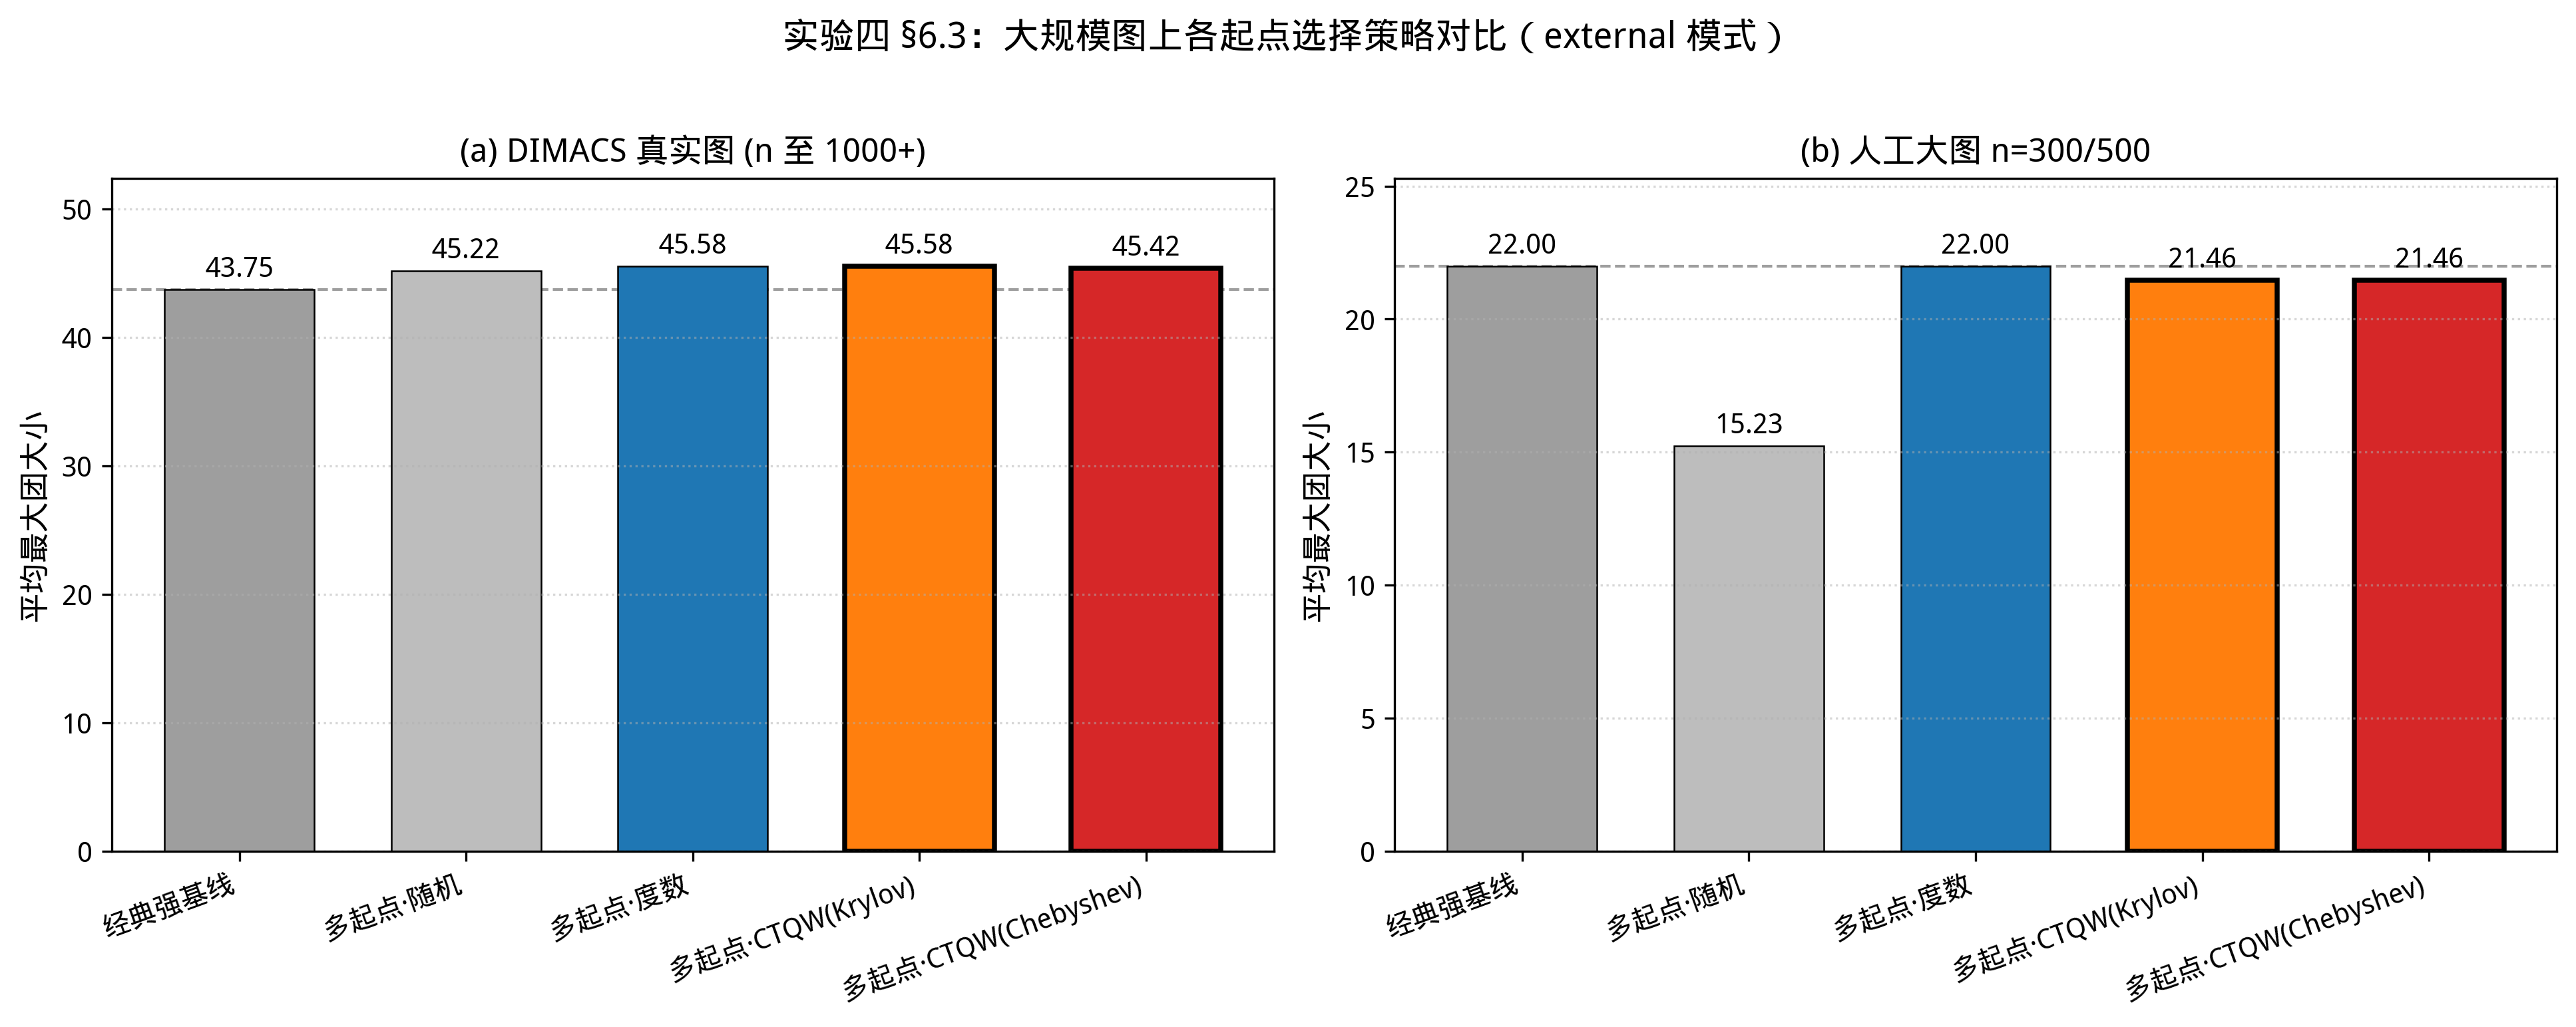
\includegraphics[keepaspectratio,alt={图 6-1：大规模图上各起点选择策略对比。左 (a) 为 DIMACS 真实图，右 (b) 为人工大图 n=300/500；虚线为经典强基线 ClassicalClique 水平，橙/红为 CTQW 两种近似。}]{figures/exp6_large_scale_comparison.png}}
\caption{图 6-1：大规模图上各起点选择策略对比。左 (a) 为 DIMACS
真实图，右 (b) 为人工大图 n=300/500；虚线为经典强基线 ClassicalClique
水平，橙/红为 CTQW 两种近似。}
\end{figure}

\begin{quote}
\textbf{图 6-1} 大规模图上各起点选择策略的平均最大团大小（external
模式）。 两个数据集上 multi-start 智能起点（度数 /
CTQW）均逼近或超过经典强基线， 而随机起点明显掉队；CTQW 的 Krylov 与
Chebyshev 两种近似结果几乎一致。
\end{quote}

\paragraph{6.3.3
嵌入式方案在大图上的复现}\label{ux5d4cux5165ux5f0fux65b9ux6848ux5728ux5927ux56feux4e0aux7684ux590dux73b0}

作为对照，我们用近似法把\textbf{嵌入式} QuantumGreedy 也跑到大规模
（embedded 模式）。DIMACS 上 QuantumGreedy(Chebyshev) 平均 41.0、
ClassicalDegree 40.8，二者接近而\textbf{双双低于 ClassicalClique
47.0}------ 实验二''嵌入式 CTQW 被度数覆盖、不及 ClassicalClique''的诊断
\textbf{在大规模真实图上依然成立}。

\subsubsection{6.4 度数误导图族上的对照（CTQW
的独有价值）}\label{ux5ea6ux6570ux8befux5bfcux56feux65cfux4e0aux7684ux5bf9ux7167ctqw-ux7684ux72ecux6709ux4ef7ux503c}

为正面检验 CTQW ``度数之外的信息''，我们构造了 \textbf{degree-misleading
数据集}
（\texttt{datasets/generate\_misleading.py}）：诱饵节点连接大量背景点以抬高度数，
但诱饵之间不连边、且每个诱饵至少缺一条到答案团的边，因此\textbf{度数最高的节点
恰恰进不了最优团}------纯度数信号在此被刻意误导。

在 30 个此类困难样本上对比（cheb\_d50，570 次运行）：

{\def\LTcaptype{none} % do not increment counter
\begin{longtable}[]{@{}ll@{}}
\toprule\noalign{}
算法 & 平均团大小 \\
\midrule\noalign{}
\endhead
\bottomrule\noalign{}
\endlastfoot
\textbf{MS\_CTQW (Chebyshev)} & \textbf{14.62} \\
MS\_HybridSeed (β=0.75) & 14.52 \\
MS\_Degree & 14.50 \\
MS\_Random & 13.86 \\
ClassicalClique 强基线 & 12.43 \\
\end{longtable}
}

\textbf{MS\_CTQW
取得全场最高均值}，是唯一在度数被误导时仍稳居第一的起点选择器。 按
(sample\_id, run\_id) 与同 K 的 MS\_Degree 配对检验：CTQW \textbf{8 胜 2
负 80 平}， 平均差
+0.12。差距虽小，但方向明确------\textbf{当度数信号失效时，CTQW 的全局
结构信号确实提供了度数之外的、可观测的额外价值}。

作为边界对照，在团节点本身度数也高的 DIMACS small3
图上，MS\_Degree（37.89） 反而略高于 MS\_CTQW（37.67），CTQW 配对 0 胜 2
负------ \textbf{进一步确认 CTQW
的相对优势只在''度数不可靠''的图族上显现}。

\subsubsection{6.5 结论}\label{ux7ed3ux8bba-1}

\begin{quote}
\textbf{实验四结论：(1) 借助 Krylov / Chebyshev 近似，CTQW
起点选择成功推广到 n=1000+ 的 DIMACS
真实图，近似精度足以保持结论、超时率为 0，大规模可行性 成立；(2)
在普通真实图与大规模 planted 图上，CTQW 与度数趋于同一水平； (3)
在专门设计的''度数误导''图族上，MS\_CTQW 取得全场最高、并在配对检验中
胜过纯度数------这是全项目中 CTQW ``度数之外价值''最直接的正面证据。}
\end{quote}

实验四把实验三的工程边界从 n≤200 推到 n≥1000，并首次在度数解耦的设定下
正面看到了 CTQW 的独立贡献，将原本属于''未来工作''的 DIMACS
解耦实验落到实处。

\subsection{7. 总结}\label{ux603bux7ed3}

\subsubsection{7.1
四组实验的最终结论}\label{ux56dbux7ec4ux5b9eux9a8cux7684ux6700ux7ec8ux7ed3ux8bba}

{\def\LTcaptype{none} % do not increment counter
\begin{longtable}[]{@{}
  >{\raggedright\arraybackslash}p{(\linewidth - 6\tabcolsep) * \real{0.2500}}
  >{\raggedright\arraybackslash}p{(\linewidth - 6\tabcolsep) * \real{0.2500}}
  >{\raggedright\arraybackslash}p{(\linewidth - 6\tabcolsep) * \real{0.2500}}
  >{\raggedright\arraybackslash}p{(\linewidth - 6\tabcolsep) * \real{0.2500}}@{}}
\toprule\noalign{}
\begin{minipage}[b]{\linewidth}\raggedright
实验
\end{minipage} & \begin{minipage}[b]{\linewidth}\raggedright
验证内容
\end{minipage} & \begin{minipage}[b]{\linewidth}\raggedright
结论
\end{minipage} & \begin{minipage}[b]{\linewidth}\raggedright
关键证据
\end{minipage} \\
\midrule\noalign{}
\endhead
\bottomrule\noalign{}
\endlastfoot
\textbf{实验一} & CTQW 能否识别图的全局团结构？ & \textbf{✓ 成立} &
Ratio = 7.08 \\
\textbf{实验二} & 嵌入式 CTQW 是否在贪心中稳健？ & \textbf{⚠ 部分成立} &
混合 \textgreater{} 单一量子（+43\%），但 \textless{}
单一经典（−6.8\%） \\
\textbf{实验三} & CTQW 外置作起点选择器，能否超越强基线？ & \textbf{✓
成立} & small/medium 均 p\textless0.001 显著胜出 \\
\textbf{实验四} & 近似推广到大规模真实图后量子信号是否仍有价值？ &
\textbf{✓ 大规模可行 + 度数误导下成立} & DIMACS 全
MS\textgreater 基线、0 超时；误导图上 MS\_CTQW 全场最高 \\
\end{longtable}
}

\textbf{三组成立，一组部分成立}。

\subsubsection{7.2 核心发现}\label{ux6838ux5fc3ux53d1ux73b0}

整个项目最关键的发现是：

\begin{quote}
\textbf{CTQW
的全局识别能力本身是真实可靠的，但其有效性高度依赖于具体的使用方式}：

\begin{itemize}
\tightlist
\item
  将其置于贪心算法\textbf{外部}、保留全图均匀叠加初态，
  能够稳定超越最强经典基线（实验三）；
\item
  将其嵌入贪心算法\textbf{内部}、改用种子集合均匀叠加初态，
  则会被经典度数评分覆盖、反而拖累整体表现（实验二）。
\end{itemize}

这两种用法对应 CTQW 的两种完全不同的物理模式------ \textbf{全局拓扑识别
vs 局部种子扩散}。
\end{quote}

这是原始理论文档中未曾明确指出的一条诊断结论，
也为后续研究指明了清晰的方向。

实验四进一步补充了两点：\textbf{工程上}，Krylov / Chebyshev
近似让上述''外部 起点选择''范式可扩展到 n=1000+
的真实图；\textbf{科学上}，在专门构造的''度数 误导''图族上，CTQW
取得全场最高并在配对检验中胜过纯度数------ 这是 CTQW
``度数之外价值''迄今最直接的正面证据， 也指明 CTQW
的用武之地在于''度数信号不可靠''的图族。

\subsubsection{7.3
后续可探索方向}\label{ux540eux7eedux53efux63a2ux7d22ux65b9ux5411}

本节列出 4 个\textbf{具体、可独立实现、互不依赖}的优化方向。
所列优化均不影响第 3-6 章已有的实验结果与结论。

\paragraph{7.3.1 方向 A：去均匀基线的 Q
评分}\label{ux65b9ux5411-aux53bbux5747ux5300ux57faux7ebfux7684-q-ux8bc4ux5206}

\textbf{改动位置}：\texttt{src/scoring.py} 的
\texttt{QuantumScorer.score\_all} 方法 \textbf{改动内容}：将原始 P\_v(t)
改为 P\_v(t) − 1/n，让''无信息节点''为零， 提升 Q 评分的对比度。

\paragraph{7.3.2 方向 B：用 Q
作为打破平局的二级排序}\label{ux65b9ux5411-bux7528-q-ux4f5cux4e3aux6253ux7834ux5e73ux5c40ux7684ux4e8cux7ea7ux6392ux5e8f}

\textbf{改动位置}：\texttt{src/algorithms/quantum\_greedy.py} 的
\texttt{solve} 方法 \textbf{改动内容}：先按 R 排序，仅当 R 相同时用 Q
决胜负------ 让 Q 评分\textbf{只在 R 无法区分时起作用}，不破坏 R
的好决策。

\paragraph{7.3.3 方向 C：多时间平均的 Q
评分}\label{ux65b9ux5411-cux591aux65f6ux95f4ux5e73ux5747ux7684-q-ux8bc4ux5206}

\textbf{改动位置}：\texttt{src/scoring.py} 的
\texttt{QuantumScorer.score\_all} 方法 \textbf{改动内容}：用多个 t
值的概率求平均（如 t ∈ \{0.5, 1, 2, 5\}）， \textbf{抹掉单 t
下的相位抖动}。

\paragraph{7.3.4 方向
D：解耦初始态，每轮都用全图均匀叠加}\label{ux65b9ux5411-dux89e3ux8026ux521dux59cbux6001ux6bcfux8f6eux90fdux7528ux5168ux56feux5747ux5300ux53e0ux52a0}

\textbf{改动位置}：\texttt{src/algorithms/quantum\_greedy.py} 的
\texttt{\_compute\_ctqw\_probs} 方法
\textbf{改动内容}：直接构造全图均匀叠加，绕开
\texttt{build\_initial\_state}------
把实验一证明有效的''全局识别初态''搬进贪心，让 λ 扰动项传递 S 的影响。

\begin{quote}
\textbf{关于原''方向 E''（DIMACS 真实图上的 CTQW vs Degree 解耦实验）}：
该方向已在\textbf{实验四}中落实------大规模 DIMACS 对比表明 CTQW
与度数趋于一致， 而专门构造的度数误导图族则首次正面展示了 CTQW
的独立价值。详见第 6 章。
\end{quote}

\subsection{8.
附录：实验运行总量}\label{ux9644ux5f55ux5b9eux9a8cux8fd0ux884cux603bux91cf}

本次工作累计运行算法实验约 \textbf{23,000 次}，分布如下：

{\def\LTcaptype{none} % do not increment counter
\begin{longtable}[]{@{}lllll@{}}
\toprule\noalign{}
实验 & 任务 & 规模 & 运行次数 & 耗时 \\
\midrule\noalign{}
\endhead
\bottomrule\noalign{}
\endlastfoot
实验一 & MC & n=30 单图 & 1 & \textless1s \\
实验二（嵌入式对比） & MC & n=30, 50 & 1040 & 6s \\
实验二（参数扫描 small） & MC & n=30, 50 & 2860 & 14s \\
实验二（参数扫描 medium） & MC & n=60\textasciitilde200 & 1680 & 526s \\
实验二（组件消融） & MC & n=30, 50 & 1040 & 3s \\
实验二（参数敏感性） & MC & n=30 单图 & \textasciitilde200 & 2s \\
D1 DS small & DS & n=30, 50 & 2880 & 17s \\
实验三（small K 扫描） & MC & n=30, 50 & 4160 & 6s \\
实验三（medium K=10） & MC & n=60\textasciitilde200 & 1680 & 89s \\
实验二（α 分层细分诊断） & MC & n=100\textasciitilde200 & 1680 & --- \\
实验四（external DIMACS） & MC & n 至 1000+ & 195 & 0 超时 \\
实验四（external 人工大图） & MC & n=300, 500 & 1700 & 0 超时 \\
实验四（embedded DIMACS） & MC & n 至 1000+ & 75 & 0 超时 \\
实验四（embedded 人工大图） & MC & n=300, 500 & 500 & 0 超时 \\
实验四（度数误导图族） & MC & n=100\textasciitilde300 & 570 & 0 超时 \\
实验四（DIMACS small3 对照） & MC & DIMACS & 57 & 0 超时 \\
\end{longtable}
}

所有结果保存在 \texttt{results/} 目录下对应子目录。

\emph{报告版本：v3.0} \emph{完成日期：见 git 提交记录}

\end{document}
